\documentclass[main.tex]{subfiles}

\begin{document}

\tableofcontents

\section{Force Interactions}

A \gls{force} is a push or a pull. Examples of a force include the push you give a car to get it moving, the \href{https://youtu.be/gzCXowhks80?t=3}{magnetic force}, and the \href{https://youtu.be/E9oKEJ1pXPw}{gravitational force}. Force is a vector: it's represented by an arrow with a direction and a magnitude that is measured in units of newtons (N). Forces act on an object or system. 

\subsection{Weight} \label{CWxEgd}

So far, we have seen only horizontal forces. Forces also apply in vertical directions. See the following.

\begin{example} \label{ex:weightIntro} 
A bowling ball is dropped from rest from the top of a cliff. (a) What is the ball's acceleration? (\textit{Hint}: Recall Unit 3: Projectiles.) (b) If the ball's mass is \SI{5}{kg}, what is the net force on it?
\end{example}

\Solution

\begin{center}
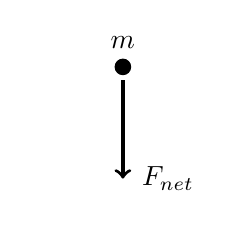
\begin{tikzpicture}
\pgfplotsset{compat=1.11}
\def\s{10}
    \begin{axis}[
        width=4cm, height=3cm,
        axis line style={draw=none},
        ticks=none,
        axis lines=middle,
        ymin=-\s, ymax=0,
        xmin=-\s, xmax=\s,
        clip=false,
    ]
    \fill (0,0) circle (3pt) node[above=3pt] {$m$};
    \draw[very thick,black,->] (0,-1.2) -- (0,-10) node[right=3pt] {$F_{\text{net}}$};
    \end{axis}
\end{tikzpicture}
\end{center}

(a) As discussed in the previous unit, the object accelerates downward due to gravity at a rate of 

\begin{equation*}
    a = -g = -\SI{9.8}{m/s^2}\ .
\end{equation*}

(b) By Newton's 2nd law (Eq.~\ref{eq:NewtonIILaw}), the net force is

\begin{equation*}
    \vec{F}_{\text{net}} = m a = -m g = -(5)(9.8) = -\SI{49}{N}\ .
\end{equation*}

Therefore, the force of gravity on the bowling ball is \SI{49}{N} downward. This result---that the magnitude of the force of gravity on an object is $mg$---is important, because this force is always present on the object, whether the object is in free-fall or not. We call it weight.

\Gls{weight} ($w$) is the downward force of gravity on an object of mass $m$:

\begin{equation} \label{eq:weight} 
    w = mg
\end{equation}

\begin{center}
    \begin{tabular}{cl|cl}
    \hline
    \textbf{Symbol} & \textbf{Quantity} & \textbf{SI Base Unit} & \textbf{Unit Symbol}  \\
    \hline\hline
    \rule{0pt}{2.5ex}
        $w$ & weight & newton & N\\
        $m$ & mass & kilogram & kg\\
        $g$ & acceleration due to gravity & meter per second squared & \SI{}{m/s^2}\\
    \hline
    \end{tabular}
\end{center}

Gravitational acceleration is $g = \SI{9.8}{m/s^2}$. It's no surprise that the equation for weight (Eq.~\ref{eq:weight}) looks like Newton's Second Law (Eq.~\ref{eq:NewtonIILaw}), as we use the latter in Example~\ref{ex:weightIntro} to derive the former. 

\vspace{1em}

\cyanhrule

\subsection{Newton's Third Law of Motion} \label{N3R3iq}

\Gls{NIIIL} states that when one object exerts a force on a second object, the first object experiences a force that is equal in magnitude and opposite in direction to the force that it exerts.

\vspace{1em}

An application of Newton's Third Law is the \gls{normal force} ($F_{\text{N}}$), which is the force that a surface applies to an object. For example, the normal force is the upward force that a table exerts on a book to support the book's weight.

\begin{example} \label{A8Qdlc}
Consider a box with a mass of \SI{7}{kg} at rest on a table. What is the magnitude of the normal force on the box? 
\end{example}

\Solution The box's weight, by Eq.~(\ref{eq:weight}), is

\begin{equation*}
    w = m g = (7)(9.8) = \SI{68.6}{N}\ .
\end{equation*}

Through its weight, the box applies a downward force of \SI{68.6}{N} on the table. Since the box is not moving, all forces on it must be balanced ($F_{\text{net}} = 0$). In other words, the box is in equilibrium. To maintain this equilibrium, the table must exert, according to Newton's Third Law, a force that is equal to the box's weight (\SI{68.6}{N}) but in the upward direction. We call this force the normal force.

\begin{center}
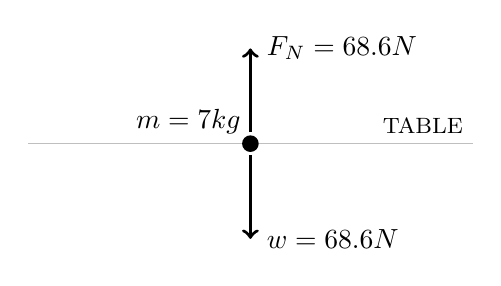
\begin{tikzpicture}
\pgfplotsset{compat=1.11}
\def\s{10}
    \begin{axis}[
        width=4cm, height=4cm,
        axis line style={draw=none},
        ticks=none,
        axis lines=middle,
        ymin=-\s, ymax=\s,
        xmin=-15, xmax=15,
        clip=false,
    ]
    \draw[lightgray] (-35,0) -- (35,0) node[above left,black] {\footnotesize TABLE}; 
    \fill (0,0) circle (3pt) node[above left] {$m = \SI{7}{kg}$};
    \draw[very thick,black,->] (0,+1.2) -- (0,+10) node[right=2pt] {$F_{\text{N}} = \SI{68.6}{N}$};
    \draw[very thick,black,->] (0,-1.2) -- (0,-10) node[right=2pt] {$w = \SI{68.6}{N}$};
    \end{axis}
\end{tikzpicture}
\end{center}

\cyanhrule

\subsection{Newton's First Law of Motion} \label{XeoZti}

\begin{mdframed}[backgroundcolor=black!10]
\gls{NIL} is summarized in 3 facts:
\vspace{-1ex}

\begin{enumerate}
\setlength\itemsep{0ex}
    \item An object at rest stays at rest.
    \item An object in motion stays in motion in a straight line at a constant speed.
    \item Facts 1 and 2 above cease being true when the object is acted upon by a net (unbalanced) force.
\end{enumerate}
\end{mdframed}

Fact 1 is obvious. Fact 2 is rarely observable on Earth, because of net forces stated in Fact 3, but it's exemplified by an asteroid or the \href{https://voyager.jpl.nasa.gov/mission/status/}{Voyager spacecrafts}. When addressing Newton's laws of motion, we may need to refer to the mass or inertia of the object. \Gls{mass} is the amount of matter in an object. It's measured in kilograms (kg). 1 kilogram is about 2.2 pounds. \Gls{inertia} is the tendency of an object to remain at rest or in motion. For example, once released, a bowling ball will tend to stay in motion. There are many examples of inertia in sports, as when players fall by their overwhelming tendency to stay in motion; see \href{https://youtu.be/5PKXs8i_zSw?t=21}{soccer}, \href{https://youtu.be/4TgpW0WZZ6U?t=55}{football}, and \href{https://youtu.be/IGBpvIXGMYQ?t=26}{basketball}. Inertia is proportional to the object's mass: if mass increases, inertia increases.

\begin{example}
Two objects---an airplane and a person---travel on a runway each at a speed of 3 meters per second. Which object has more inertia?
\end{example}

\Solution Inertia is proportional to mass. The airplane, with its vastly greater mass, has more inertia. Furthermore, it's easy to stop a person in their tracks; good luck trying to stop a \SI{400000}{lbs.} Boeing 747.

\solutionEnd

\vspace{1em}

\cyanhrule


\subsection{Exercises}

\subsubsection*{Weight}

\begin{exercise}
Compare weight and mass. (a) What are the units of weight? (b) What are the units of mass? (c) Are mass and weight the same thing? (d) Which is always constant? and which may change? (\textit{Hint}: Astronauts in space are said to be ``\href{https://youtu.be/C3GC5LS6e6Q}{weightless}.'')
\end{exercise}

\begin{exercise} \label{eStk9M}
What is the weight of a box with a mass of \SI{10}{kg}?
\end{exercise}

\begin{exercise} \label{x9Ufbz}
A 44-kilogram person has a weight of \rule{1cm}{0.15mm} newtons.
\end{exercise}

\begin{exercise} \label{r7dwXZ}
An adult grizzly bear can ``weigh'' up to \SI{300}{kg}---that's actually its \textit{mass}. What is the weight of the bear, in newtons, as we have defined it above?
\end{exercise}

\begin{exercise} \label{neLJbr}
What is the mass of a dumbbell whose weight is \SI{2450}{N}? (\textit{Hint}: Review the solution to Example~\ref{ex:Solve_NIIL_a}.)
\end{exercise}

\subsubsection*{Newton's Third Law}

\begin{exercise} \label{f03y7Z}
    Suppose you are installing a smoke detector in the ceiling of your house. You push up on the detector to snap it into place. What is the direction of the normal force exerted by the ceiling on the detector?
\end{exercise}

\begin{exercise} \label{BkOxdJ}
Judy, whose mass is \SI{60}{kg}, lays down on a park bench. What is the normal force by the bench on Judy?
\end{exercise}


\begin{exercise} \label{QaZUiq}
What is the magnitude and direction of the normal force on a \SI{100}{kg} container at rest on a table?
\end{exercise}

\begin{exercise} \label{wkga6W}
Consider the \SI{7}{kg} box from Example \ref{A8Qdlc}. (a) Re-draw the free-body diagram to show a person pushing down on the box with a force of \SI{84}{N}. (b) What is the normal force on the box now?
\end{exercise}

\begin{exercise} \label{hIgPqQ}
Ben, the 80-kilogram zookeeper is standing on a platform at the zoo. (a) Draw a free-body diagram including Ben's weight and the normal force on him. (b) What is the magnitude of the normal force on Ben? (c) If he picks up a container of water weighing \SI{215}{N}, what is the normal force exerted by the platform now? 
\end{exercise}

\begin{exercise} \label{SwLQsz}
    Bob is at the gym. He sees a \SI{65}{kg} dumbbell at rest on a rack and tries to pick it up, but he applies only a 500-newton upward force on the weight. (a) Draw a free-body diagram of Bob's feeble attempt to lift the weight. (b) The instant the upward force is exerted, what is the normal force of the rack on the dumbbell?
\end{exercise}

\subsubsection*{Newton's First Law}

\begin{exercise} \label{prob:fgm}
In your own words summarize Newton's First Law of Motion. Given some examples of each fact of the First Law. 
\end{exercise}


\begin{exercise} \label{WTFwXI}
According to Fact 2 of Newton's First Law, it's expected that when you let go of a shopping cart it will continue traveling at a constant speed in one direction forever. From experience, however, we know that the shopping cart always comes to a stop. (a) Does this observation violate Newton's First Law of Motion? (b) What causes the shopping cart to come to rest? (\textit{Hint}: See Fact 3.)
\end{exercise}

\begin{exercise} \label{MB3Xar}
If you’re ever being chased by a bear, it’s recommended that you run in zig-zags rather than in a straight line. A zig-zag motion decreases the probability that the bear will catch you. (a) How does the inertia of the bear compare to yours? (b) How does the concept of inertia explain the recommendation stated above? (\textit{Hint}: Refer to Newton's First Law of Motion.)
\end{exercise}

\subsection{Answers to Exercises}

\ref{eStk9M}. \SI{98}{N}\\
\ref{x9Ufbz}. \SI{431.2}{N}\\
\ref{r7dwXZ}. \SI{2940}{N}\\
\ref{neLJbr}. \SI{250}{kg}\\
\ref{f03y7Z}. Down\\
\ref{BkOxdJ}. \SI{588}{N}\\
\ref{QaZUiq}. \SI{980}{N}\\
\ref{wkga6W}. \SI{152.6}{N}\\
\ref{hIgPqQ}. (b) \SI{784}{N} \hspace{1em} (c) \SI{999}{N}\\
\ref{SwLQsz}. (b) \SI{137}{N}\\


\end{document}


